% Copyright (c) 2021 Eclipse Arrowhead Project
%
% This program and the accompanying materials are made available under the
% terms of the Eclipse Public License 2.0 which is available at
% http://www.eclipse.org/legal/epl-2.0.
%
% SPDX-License-Identifier: EPL-2.0

The \GlossaryHyperRef{framework-arrowhead}{Arrowhead framework}, which is illustrated in Figure \ref{fig:framework}, consists of two subframeworks: a \GlossaryHyperRef{framework-idea}{framework of ideas} and a \GlossaryHyperRef{framework-software}{framework of software}.
The framework of ideas formulates and frames the \GlossaryHyperRef{domain-problem}{\textit{problem domain}} the framework of software is meant to help address.
By this we mean that the framework of ideas presents the \GlossaryHyperRef{assumption}{assumptions}, \GlossaryHyperRef{concept}{concepts}, \GlossaryHyperRef{value}{values} and \GlossaryHyperRef{practice}{practices} that should be applied when \GlossaryHyperRef{specification}{specifying} \GlossaryHyperRef{architecture}{architectural} or other technical documentation and when \GlossaryHyperRef{implementation}{implementing} any kinds of Arrowhead systems or components.

\begin{figure}[ht!]
  \centering
  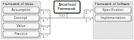
\includegraphics[scale=0.9]{figures/framework}
  \caption{
    The two subframeworks of the Arrowhead framework, concerned with \textit{ideas} and \textit{software}.
    The specifications and implementations of the software framework must conform to the assumptions, concepts, values and practices of the idea framework.
    The concepts of the idea framework are outlined in this document.
  }
  \label{fig:framework}
\end{figure}

This document is part of Arrowhead's framework of ideas.
As such, it is primarily concerned with defining concepts.
However, before we move on to consider our overview those concepts, we will first present a few examples of other key framework ideas.\footnote{
  At the time of writing, the best source of assumptions, values and practices of the Arrowhead framework is Jerker Delsing's book \textit{{IoT} Automation: Arrowhead Framework} \cite{delsing2017iot}.
  The \GlossaryHyperRef{project-eclipse-arrowhead}{Eclipse Arrowhead project} may publish other works of relevance in the future.
}
It is, for example, \textit{assumed} that the framework may be applied in contexts where the primary activity is markedly physical, such as in transportation, mining, manufacturing, electricity generation, healthcare, and so on.
One of the system characteristics \textit{valued} by the framework is \textit{resilience}, or the expectation that every system should do its outmost to mitigate and recover from degradations, failures or other contingencies that may affect its ability to perform its designated tasks.
Finally, one of its \textit{recommended practices} is that every system-of-systems should be thoroughly documented at every level, from its smallest components up to its most high-level interactions.

The rest of this section gives an overview of the most fundamental concepts of the framework.
It is meant to prepare you for the next section, where the same concepts, and other supporting concepts, are presented in greater detail.

\subsection{Stakeholders and Artifacts}

There are two kinds of members of the world of Arrowhead, (1) \GlossaryHyperRef{stakeholder}{stakeholders} and (2) \GlossaryHyperRef{artifact}{artifacts}, as depicted in Figure \ref{fig:world}.
The former denotes a \GlossaryHyperRef{person}{person} or \GlossaryHyperRef{organization}{organization} engaged in an Arrowhead enterprise, while the latter is any thing or object, tangible or intangible, that could be relevant to consider as part of such an enterprise.
Stakeholders \GlossaryHyperRef{owner}{own}, \GlossaryHyperRef{supplier}{supply}, \GlossaryHyperRef{developer}{develop}, \GlossaryHyperRef{operator}{operate}, and \GlossaryHyperRef{user}{use} artifacts, among many other possible activities.
It is their business needs and ambitions that govern what and how Arrowhead artifacts are employed.

\vfill

\begin{figure}[ht!]
  \centering
  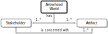
\includegraphics[scale=0.9]{figures/world}
  \caption{
    The two kinds of members of the Arrowhead world: stakeholders and artifacts.
  }
  \label{fig:world}
\end{figure}

\subsection{Devices, Systems and Services}

The most essential types of artifacts in the world of Arrowhead are (1) \GlossaryHyperRef{device}{hardware devices}, (2) \GlossaryHyperRef{system}{software systems} and (3) \GlossaryHyperRef{service}{services}, all shown in Figure \ref{fig:device-system-service}.
\textit{Hardware devices}, or just \textit{devices}, are physical machines, such as servers, robots or tools, that are able to maintain, or \GlossaryHyperRef{hosting-system}{\textit{host}}, \textit{software systems}.
A software system, or just \textit{system}, is a \GlossaryHyperRef{communication}{communicating} \GlossaryHyperRef{instance-software}{software instance} that \GlossaryHyperRef{provision-service}{provides} \textit{services}.
Every service represents a set of tasks a system can perform for other systems or for its stakeholders.
When a system or stakeholder makes use of a service, it is said to \GlossaryHyperRef{consumption-service}{\textit{consume}} it.

\vfill

\begin{figure}[ht!]
  \centering
  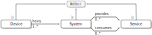
\includegraphics[scale=0.9]{figures/device-system-service}
  \caption{
    Hardware devices \textit{host} software systems, which \textit{consume} and/or \textit{provide} services.
  }
  \label{fig:device-system-service}
\end{figure}

\vfill

Every service represents one area of concern its hosting system can address.
Examples of such areas of concern could be generating financial statements, replacing propellers on drones, manufacturing bolts or measuring humidity.
A service providing control over a door could, for example, make it possible to check if the door is open, to open it and to close it.
Each such activity of every service is represented by one \GlossaryHyperRef{operation}{service operation}, which we will consider more in the next section.

\subsection{Service Provision and Consumption}

As we have already established, \GlossaryHyperRef{communication}{communication} between systems is formulated in terms of the \GlossaryHyperRef{provision-service}{provision} and \GlossaryHyperRef{consumption-service}{consumption} of \GlossaryHyperRef{service}{services}.
\GlossaryHyperRef{system}{Systems} may \textit{provide} services, which other systems can \textit{consume} by sending \GlossaryHyperRef{message}{messages} to their \GlossaryHyperRef{operation}{operations}, as depicted in Figure \ref{fig:service-consumption}.

\vfill

\begin{figure}[ht!]
  \centering
  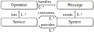
\includegraphics[scale=0.9]{figures/service-consumption}
  \caption{
    Systems consume services by sending messages to the providers of those services.
    Those providers then pass on the messages they receive to their service operations, which interpret and handle them.
  }
  \label{fig:service-consumption}
\end{figure}

\vfill

Also \GlossaryHyperRef{person}{persons} can consume services, even though it is not explicitly depicted in Figure \ref{fig:service-consumption}.
This, however, requires that a \GlossaryHyperRef{interface-human}{human interface} is attached to the providing system, or that another system with such an interface can act as \GlossaryHyperRef{proxy}{proxy}.
The human interface enables the person, via its buttons, prompts or other elements, to send messages to the services in question, just as a regular system would.

When a providing system receives a message from a consuming system or person, it passes it on to the service operation specified in that message, as described in Sections \ref{sec:concepts:service} and \ref{sec:concepts:interface}.
The operation receiving the message will then handle it by performing whatever action it describes, given that the message is \GlossaryHyperRef{message-valid}{valid} and \GlossaryHyperRef{message-permitted}{permitted}.
This handling may entail sending additional messages to other systems, starting or stopping various kinds of automation routines, reading from sensors, electronically signing contracts, sending notifications to an \GlossaryHyperRef{operator}{operator}, sending one or more messages back to the sender, among many other possible examples.

\subsection{System Composition}
\label{sec:overview:system-composition}

\GlossaryHyperRef{system}{Systems} will typically \GlossaryHyperRef{consumer-service}{consume services} because it is a necessary part of executing the tasks they were designed to perform.
Consider, for example, a scenario in which a number of automated guided vehicles, each of which is a system, are to move items around a factory as directed by a scheduling system.
As the scheduling system does not have wheels, engines or other necessary sensors and actuators, it cannot physically move any items by itself. 
Likewise, the individual vehicles are not capable of themselves deciding what needs to be taken to what location.
However, the combination of a scheduling system and vehicles becomes able to plan, track and execute the moving of items.
When these systems cooperate by consuming each others' services, they become able to do things none of them could by themselves.
When systems consume each other's services in this manner, they form a so-called \GlossaryHyperRef{system-of-systems}{system-of-systems}.

As depicted in Figure \ref{fig:systems-of-systems}, there are different kinds of systems-of-systems with their own characteristics.
There are \GlossaryHyperRef{cloud}{clouds} and \GlossaryHyperRef{system-of-clouds}{systems-of-clouds}, as well as \textit{local} and \textit{virtual} variants of both.\footnote{
  In addition to being local or virtual, a cloud may also be \textit{Arrowhead-compliant}.
  Such a cloud is referred to as an \GlossaryHyperRef{cloud-arrowhead}{\textit{Arrowhead cloud}} and conforms to various architectural requirements put forth by the \GlossaryHyperRef{project-eclipse-arrowhead}{Eclipse Arrowhead project} in a separate document.
}

\vfill

\begin{figure}[ht!]
  \centering
  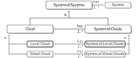
\includegraphics[scale=0.9]{figures/systems-of-systems}
  \caption{
    The different kinds of \textit{systems-of-systems}, each of which consists of a number of \textit{systems} that consume each others' services.
    Clouds are systems-of-systems with \textit{boundaries} and \textit{resource pools}, while systems-of-clouds combine multiple clouds.
  }
  \label{fig:systems-of-systems}
\end{figure}

\vfill

When a system-of-systems has at least one \GlossaryHyperRef{boundary-cloud}{boundary} and at least one pool of \GlossaryHyperRef{resource}{resources}, we refer to it as a \textbf{cloud}.
Boundaries may be formed via access control policies, firewalls, gateway systems, physical separation, among many other possible examples.
Pools of resources may consist of mining equipment, \GlossaryHyperRef{unit-compute}{compute units}, sand, or whatever else is used by the cloud in question to render its services.
Because the Arrowhead framework is highly concerned with physical automation processes, we distinguish \GlossaryHyperRef{cloud-local}{local clouds} from \GlossaryHyperRef{cloud-virtual}{virtual clouds}.

The \textbf{local cloud} has \GlossaryHyperRef{boundary-local}{local boundaries} and \GlossaryHyperRef{resource-local}{local resources}, which means that it must be associated with a physical location.
Examples of local clouds could be smelting stations, drone control towers, assembly lines, power distribution centers, or the components of a satellite.
Whether it be ore, drones, parts, power cables or a complex mesh of all those things, the resources of these example clouds are all markedly \textit{physical}.
Because of their physicality, it matters \textit{where} the clouds are physically located.
Since physical isolation is a form of physical boundary, each of them has both at least one local boundary and at least one local resource.

On the other hand, a \textbf{virtual cloud} has only \GlossaryHyperRef{boundary-virtual}{virtual boundaries} and \GlossaryHyperRef{resource-virtual}{virtual resources}, which means that the values produced by the cloud are not tied to its physical location.
This is the kind of cloud that underpins much of the modern Internet.
A few companies let out virtual compute, storage and network resources, which their clients rent to provision their own virtual clouds and provide their own virtual services.
A virtual cloud could provide services for forecasting, analysis, design, planning, communication, or digital entertainment, among other possible examples.

Individual clouds may be interconnected to former even larger systems-of-systems, which we then refer to as \textbf{systems-of-clouds}.
The individual clouds may be owned and operated by different departments, subdivisions or teams at the same company, or even by different legal entities.
Some of them may be local, while other may be virtual.
Examples of systems-of-clouds may be a set of weather stations operated by the same company, the robots of distinct collaborating companies at a mining site, or the carriers of a supply chain.
When a system-of-clouds contain only local clouds, we refer to it as a \GlossaryHyperRef{system-of-local-clouds}{systems-of-local-clouds}.
Likewise, a system-of-clouds with only virtual clouds constitute a \GlossaryHyperRef{system-of-virtual-clouds}{systems-of-virtual-clouds}.
